% tex file for regression results
\par To develop linear models, we looked at the HR from the neural response 
as a single feature and used multiple regression to take into account the 3 
different types of stimulus (pump, explode, cash-out) to see if the 
separation of these stimuli can better describe the response. Specifically, 
this allows for the prediction of different amplitudes for each type of 
stimulus's HR function in linear regression. The predictive power of these 
models was not very good [Figure \ref{fig:fit_vs_act}] [Figure \ref
{fig:all_cond_time}]. 

\begin{figure}[ht]
\centering
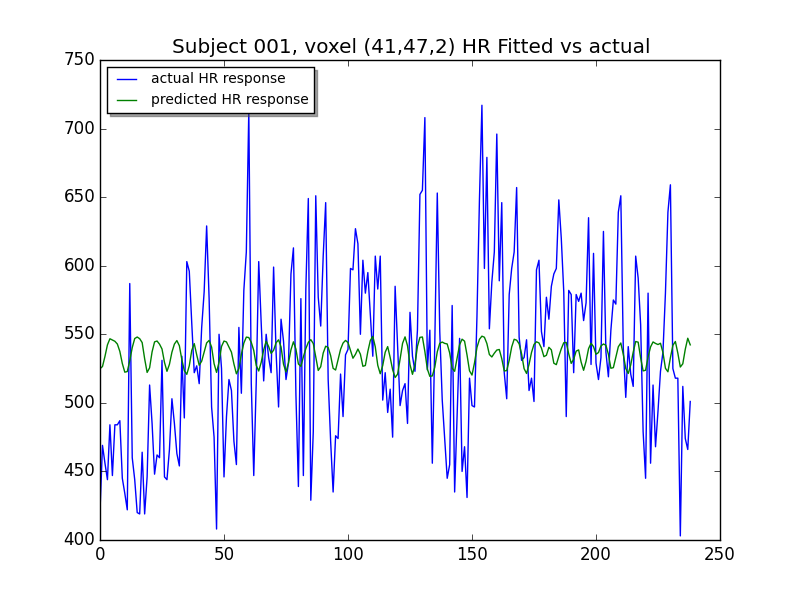
\includegraphics[scale=.5]{images/fitted_vs_actual_mult_regression}
\caption{Fitted vs observed HR based on regressions.}
\label{fig:fit_vs_act}
\end{figure}
  
\begin{figure}[ht]
\centering
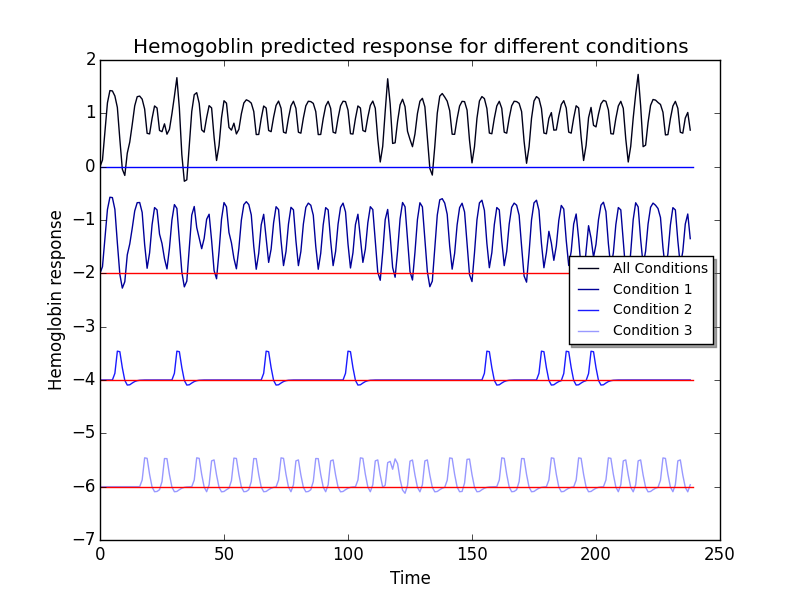
\includegraphics[scale=.5]{images/all_cond_time}  
\caption{Plotting all predicted HR for conditions.}
\label{fig:all_cond_time}
\end{figure}

As we also obtained $\hat{\beta}$ values (coefficients) from the linear 
regression models, we looked at the 3-dimensional reports of the 
$\hat{\beta}$ values, a less rigorous analysis than hypothesis testing with 
t-statistics [Figure \ref{fig:con1_beta_brain}]. 

\begin{figure}[ht]
\centering
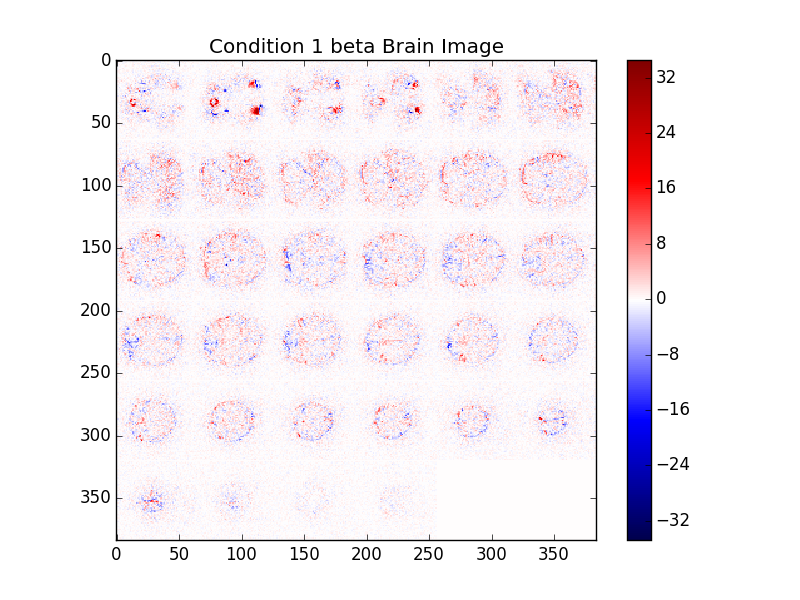
\includegraphics[scale=.5]{images/mr_cond1_beta_brain}    
\caption{$\hat{\beta}$ values for condition 1, subject 001.}
\label{fig:con1_beta_brain}
\end{figure}

The numerous other multiple regression models discussed in 
\textit{Linear Regression} should be analyzed similarly in the future. 
